\documentclass[sigconf,nonacm,pbalance]{acmart}
\usepackage{booktabs}
\usepackage{pifont}
\usepackage[shortlabels]{enumitem}
\settopmatter{printfolios=true}

\begin{document}

\title{Fast Image Search over ImageNet-1k: What Approximate Indexing and Quantization Buy}
\subtitle{CAP6938 Homework 2}

\author{Longho Bernard Che}
\affiliation{%
  \institution{University of Central Florida}
  \country{USA}}

\begin{abstract}
This project builds a search system that returns the 10 images most similar to a query image from the 1.28 million ImageNet-1k
training images. It then measures what approximate indexing and quantization gain and lose compared with exact search. An IVF index
is 105$\times$ faster than exact search with the same precision. Adding product quantization makes search 241$\times$ faster and the index
37$\times$ smaller, for a loss of 0.02 in precision.
\end{abstract}

\maketitle

\section{Introduction}

Each image is represented by an embedding vector, and the search returns the 10 database vectors closest to the query's vector.
\emph{Exact search} (Flat) compares the query with all 1.28M vectors. It is accurate but slow, and it needs about 4\,GB of memory. This
report tests two standard remedies:
\begin{itemize}[nosep,leftmargin=*]
  \item \textbf{Approximate indexing (IVF)} groups the vectors into 4{,}096 clusters and searches only the \emph{nprobe} clusters nearest to the
  query. A larger nprobe gives more accurate results but slower search.
  \item \textbf{Quantization} stores compressed vectors. SQ8 keeps 1 byte per dimension (4$\times$ smaller). PQ64 splits each 768-dimensional vector into 64 parts
  of 12 dimensions and stores, for each part, the 1-byte id of the nearest of 256 learned centroids (48$\times$ smaller).
\end{itemize}

\section{Method}

\begin{enumerate}[nosep,leftmargin=*]
  \item \textbf{Split the data.} The \emph{database} is the whole \emph{train} split (1{,}281{,}167 images, 732--1{,}300 per class). The
  \emph{queries} are one image per class drawn uniformly at random (seed 42) from the \emph{validation} split, which has 50 images per class,
  giving 1{,}000 queries. The \emph{test} split was not used because its labels are not public. Since database and queries come from different
  splits, a query never finds itself.
  \item \textbf{Embed} every image with OpenAI CLIP ViT-L/14 (768 dimensions) and normalise each vector to unit length, so the inner product
  equals cosine similarity. Embedding took 0.59\,h on a Colab A100 GPU (603 images/s).
  \item \textbf{Index} with five FAISS settings that cover exact and approximate search, each with and without quantization (Table~\ref{tab:main}).
  The IVF clusters, SQ8 value ranges and PQ centroids were learned from 200{,}000 randomly sampled database vectors, never from queries.
  IVF-PQ uses the same clusters as IVF-Flat, so the two differ only by quantization.
  \item \textbf{Measure} on a Colab CPU runtime, one query at a time. \emph{Latency} is the median and 99th percentile (p99) search time per query,
  excluding the time to embed the query. \emph{Memory} is the size of the saved index. \emph{Precision@10} (P@10) is the fraction of the top 10
  results with the query's class. \emph{Recall@10} (R@10) is the fraction of exact search's top 10 that a setting also returns; it isolates the loss
  caused by the index and quantization.
  \item \textbf{Reproduce.} Table~\ref{tab:config} lists every setting that affects the results. The three notebooks read each one from an
  environment variable, with these values as defaults.
\end{enumerate}

\begin{table}[t]
\centering\footnotesize
\setlength{\tabcolsep}{3pt}
\caption{Configuration used for all results.}
\label{tab:config}
\begin{tabular}{@{}lp{0.70\columnwidth}@{}}
\toprule
Dataset & \texttt{benjamin-paine/imagenet-1k-256x256} (Hugging Face) \\
Queries & 1 per class from \emph{validation}, random seed 42 \\
Model & \texttt{open\_clip} \texttt{ViT-L-14-quickgelu}, \texttt{openai} weights \\
Preprocessing & bicubic resize to 224\,px, centre crop, CLIP mean/std; fp16, batch 256 \\
Vectors & 768-d, L2-normalised, stored as fp16; inner-product metric \\
IVF & 4{,}096 lists; nprobe $\in\{1,2,4,\dots,128\}$, reported at 16 \\
Quantization & SQ8 (8 bits/dim); PQ 64 sub-vectors $\times$ 8 bits \\
Index training & 200{,}000 database vectors, random seed 42 \\
Search & top 10; 50 untimed warm-up queries; 1 query per call \\
Failure rule & P@10 bad $\le$\,0.3, good $\ge$\,0.7, drop $\ge$\,0.3 \\
Software & Python 3.13, PyTorch 2.11, \texttt{open\_clip} 2.32.0, \texttt{faiss-cpu} 1.11.0 \\
Hardware & embedding: A100-SXM4-40GB; search: Colab CPU, 2 vCPUs, 2 FAISS threads \\
\bottomrule
\end{tabular}
\end{table}

\section{Results}

\begin{table}[t]
\centering\small
\setlength{\tabcolsep}{3.2pt}
\caption{Results on 1{,}000 queries, with IVF at nprobe\,=\,16. Speedup is relative to Flat's median latency.}
\label{tab:main}
\begin{tabular}{@{}lrrrrrr@{}}
\toprule
Setting & MB & Med.\,ms & p99\,ms & Speedup & P@10 & R@10\\
\midrule
Flat (exact)  & 3{,}936 & 366.4 & 454.1 & 1$\times$   & \textbf{.701} & 1.000\\
SQ8 (exact)   &    984 & 216.0 & 472.1 & 1.7$\times$ & \textbf{.701} & .981\\
PQ64 (exact)  &     83 &  45.8 &  86.5 & 8$\times$   & .606 & .329\\
IVF-Flat      & 3{,}959 &   3.5 &   6.0 & 105$\times$ & \textbf{.701} & .975\\
IVF-PQ64      &    106 &   1.5 &   2.1 & \textbf{241$\times$} & .682 & .492\\
\bottomrule
\end{tabular}
\end{table}

\begin{figure*}[t]
\centering
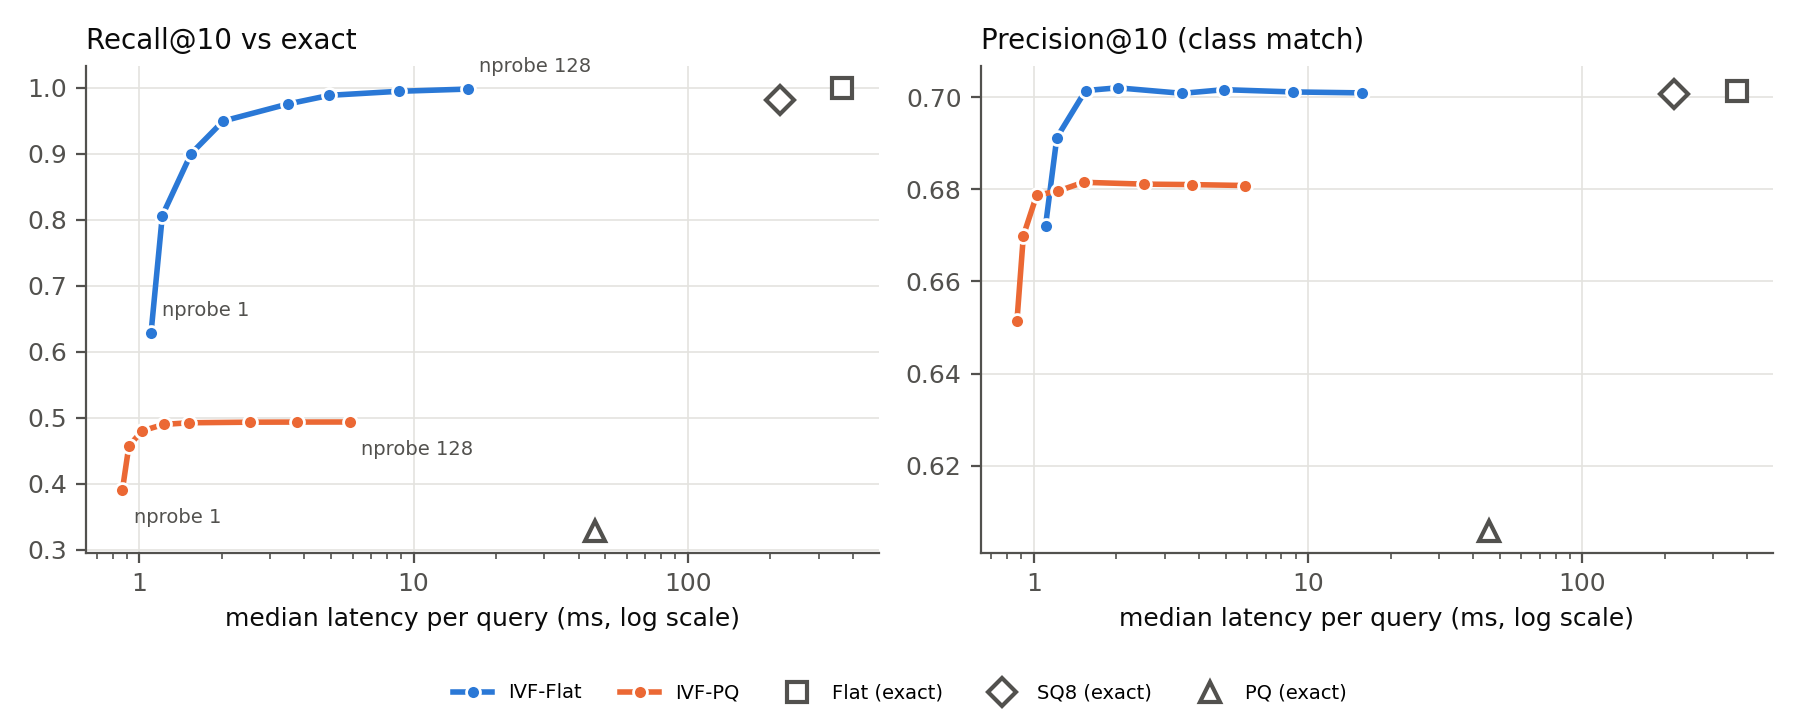
\includegraphics[width=0.62\textwidth]{figures/tradeoff.png}
\Description{Two line charts of recall@10 and precision@10 against median query latency on a log axis. IVF-Flat rises to recall near 1.0 by about 3 ms; IVF-PQ flattens at recall 0.49; exact Flat, SQ8 and PQ appear as single points at 46 to 366 ms.}
\caption{Recall@10 (left) and precision@10 (right) against median latency as nprobe grows from 1 to 128. Exact-search settings are single points.}
\label{fig:tradeoff}
\end{figure*}

\begin{figure*}[t]
\centering
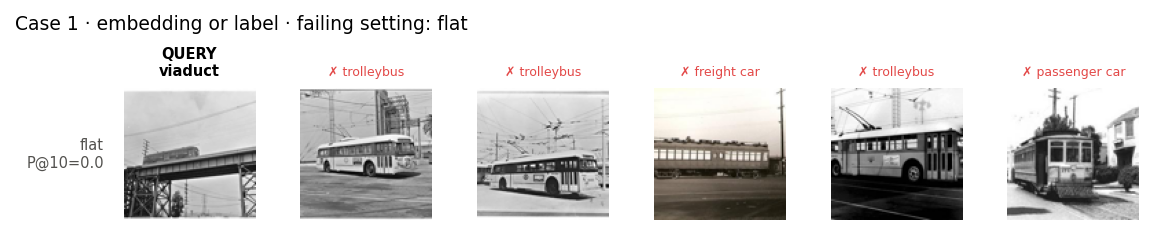
\includegraphics[width=0.495\textwidth]{figures/case1.png}\hfill
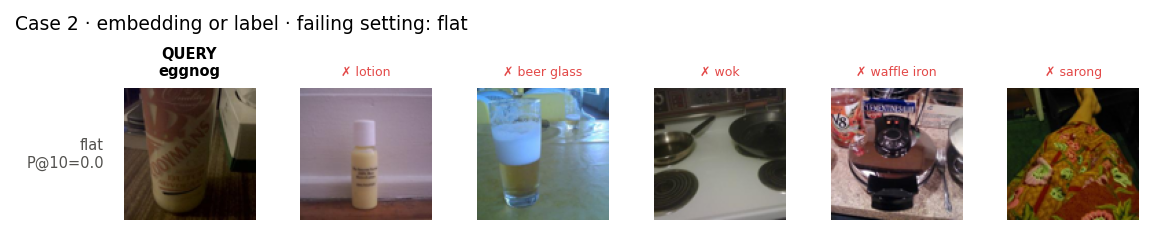
\includegraphics[width=0.495\textwidth]{figures/case2.png}\\[1pt]
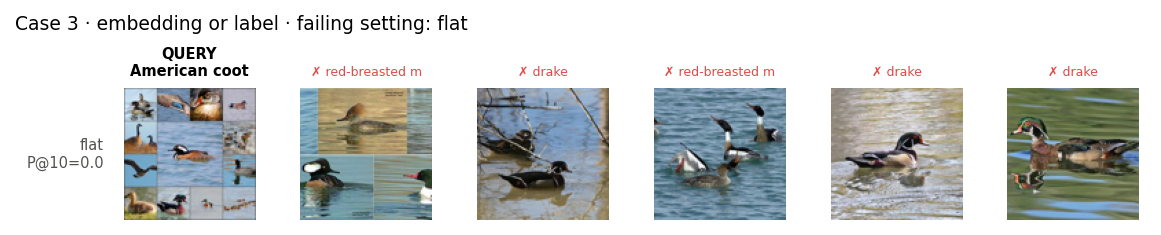
\includegraphics[width=0.495\textwidth]{figures/case3.png}\hfill
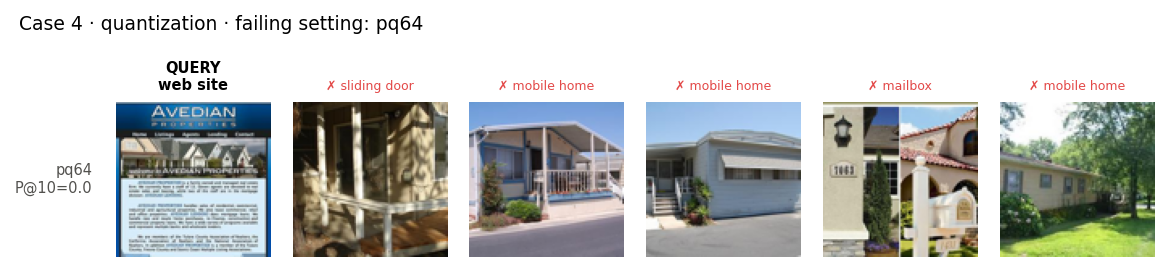
\includegraphics[width=0.495\textwidth]{figures/case4.png}\\[1pt]
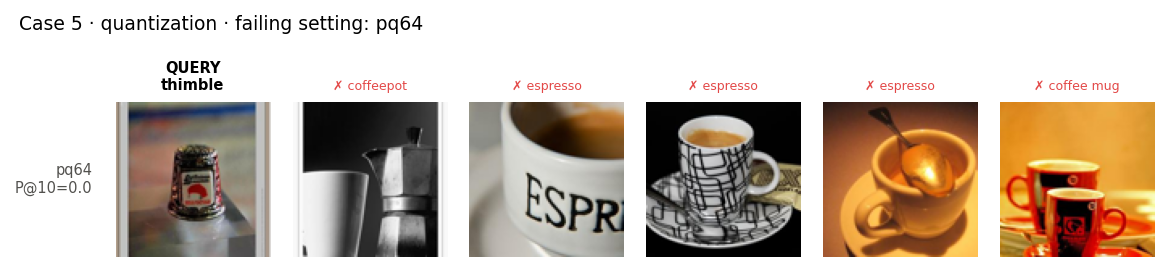
\includegraphics[width=0.495\textwidth]{figures/case5.png}\hfill
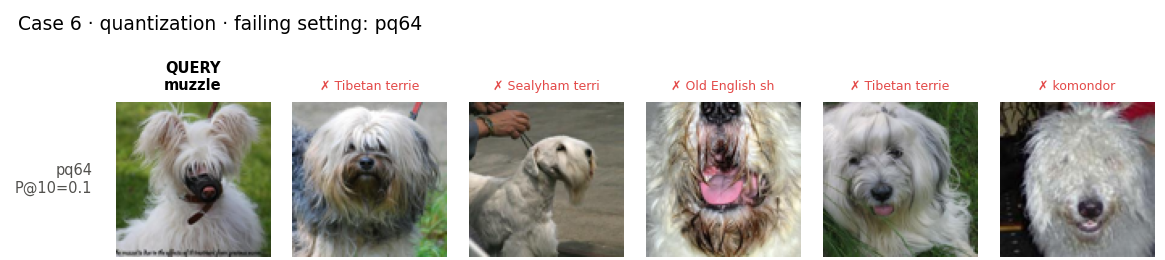
\includegraphics[width=0.495\textwidth]{figures/case6.png}
\Description{Six image strips, each showing a query image followed by its top five retrieved images labelled with their ImageNet classes: viaduct, eggnog, American coot, web site, thimble and muzzle queries.}
\caption{Failure cases: the query and the top 5 results of the failing setting (\textcolor[HTML]{e34948}{\ding{55}} = different class).
In cases 4--6, exact search returns 10/10 correct results and IVF-PQ 9--10/10.}
\label{fig:fail}
\end{figure*}

Table~\ref{tab:main} compares the five settings, and Figure~\ref{fig:tradeoff} shows how accuracy and latency change with nprobe.
\begin{enumerate}[nosep,leftmargin=*]
  \item \textbf{IVF buys speed, not memory.} At nprobe\,=\,16, IVF-Flat is 105$\times$ faster than exact search, keeps 97.5\% of its results, and has the same
  precision. Raising nprobe beyond 8--16 adds little: going from 8 to 128 lifts recall from 0.950 to 0.998 but makes search 7.8$\times$ slower.
  \item \textbf{SQ8 buys memory, not speed.} It is 4$\times$ smaller with almost the same accuracy, but only 1.7$\times$ faster, because it still compares the query with every vector.
  \item \textbf{PQ buys both, at a cost in recall.} IVF-PQ is the fastest (1.5\,ms) and nearly the smallest (106\,MB) setting, and it loses only
  0.02 precision. Its recall, however, stays near 0.49 whatever the nprobe. Quantization, not the number of clusters searched, sets that limit.
  \item \textbf{IVF-PQ beats plain PQ.} With the same 64-byte codes, IVF-PQ reaches recall 0.49, while PQ alone reaches 0.33. IVF-PQ compresses each
  vector's offset from its cluster centre, which is smaller than the vector itself and so is encoded more accurately.
  \item \textbf{Precision drops much less than recall,} because quantization usually replaces a true neighbour with another image of the same class.
\end{enumerate}

\section{Failure Analysis}

The cause of each failure was identified by comparing a query's P@10 across settings at nprobe\,=\,16:
\begin{itemize}[nosep,leftmargin=*]
  \item wrong even under exact search (P@10\,$\le$\,0.3): the \emph{embedding model} or the \emph{label};
  \item correct under exact search and IVF-Flat, but P@10 drops by $\ge$\,0.3 under PQ: \emph{quantization};
  \item P@10 drops under IVF-Flat: the \emph{approximate index}. No query fell into this group.
\end{itemize}
Figure~\ref{fig:fail} shows six cases:
\begin{enumerate}[nosep,leftmargin=*]
  \item \textbf{Viaduct (label).} A streetcar on a viaduct. The results are streetcars, which really are in the image, but ImageNet allows only one label.
  \item \textbf{Eggnog (embedding).} A dim photo of a bottle. The results share only the dark indoor look, not the object.
  \item \textbf{American coot (label).} The query is a collage of ducks with no coot in it. The returned ducks are correct.
  \item \textbf{Web site (quantization).} PQ kept the house photo on the page and lost the page layout, so it returns houses.
  \item \textbf{Thimble (quantization).} PQ placed the thimble among the much more common cup images, so it returns espresso cups.
  \item \textbf{Muzzle (quantization).} PQ kept ``white shaggy dog'' and lost the muzzle, so it returns terriers.
\end{enumerate}

\section{Conclusion}

Precision is capped at 0.70 by the embedding model, not by the index. For 214 of the 1{,}000 queries, even exact search finds 3 or fewer correct images.
If about 4\,GB of RAM is available, IVF-Flat at nprobe 8--16 gives exact-level precision in 2--3.5\,ms. If memory is limited, IVF-PQ at nprobe 8--16 needs only
106\,MB and about 1.3\,ms, for 0.02 lower precision.

\end{document}
